%
% teil1.tex -- Beispiel-File für das Paper
%
% (c) 2020 Prof Dr Andreas Müller, Hochschule Rapperswil
%
\subsection{Ordnungsstatistik und Beta-Funktion
\label{buch:rekursion:ordnung:section:ordnungsstatistik}}
In diesem Abschnitt ist $X$ eine Zufallsvariable mit der Verteilungsfunktion
$F_X(x)$ und $X_i$, $1\le i\le n$, sei ein Stichprobe von unabhängigen
Zufallsvariablen, die wie $X$ verteilt sind.
Ziel ist, die Verteilungsfunktion und die Wahrscheinlichkeitsdichte
des grössten, zweitgrössten, $k$-t-grössten Wertes in der Stichprobe
zu finden.
Wir schreiben $[n]=\{1,\dots,n\}$ für die Menge der natürlichen
Zahlen von zwischen $1$ und $n$.

\subsubsection{Verteilung von $\operatorname{max}(X_1,\dots,X_n)$ und
$\operatorname{min}(X_1,\dots,X_n)$
\label{buch:rekursion:ordnung:subsection:minmax}}
Die Verteilungsfunktion von $\operatorname{max}(X_1,\dots,X_n)$ hat
den Wert
\begin{align*}
F_{\operatorname{max}(X_1,\dots,X_n)}(x)
&=
P(\operatorname{max}(X_1,\dots,X_n) \le x)
\\
&=
P(X_1\le x\wedge \dots \wedge X_n\le x)
\\
&=
P(X_1\le x) \cdot \ldots \cdot P(X_n\le x)
\\
&=
P(X\le x)^n
=
F_X(x)^n.
\end{align*}
Für die Gleichverteilung ist
\[
F_{\text{equi}}(x)
=
\begin{cases}
0&\qquad x< 0
\\
x&\qquad 0\le x\le 1
\\
1&\qquad 1<x.
\end{cases}
\]
In diesem Fall ist die Verteilung des Maximums
\[
F_{\operatorname{max}(X_1,\dots,X_n)}(x)
=
\begin{cases}
0&\qquad x<0\\
x^n&\qquad 0\le x\le 1\\
1&\qquad 1 < x.
\end{cases}
\]
Mit der zugehörigen Wahrscheinlichkeitsdichte
\[
\varphi_{\operatorname{max}(X_1,\dots,X_n)}
=
\frac{d}{dx}
F_{\operatorname{max}(X_1,\dots,X_n)}(x)
=
\begin{cases}
nx^{n-1}&\qquad 0\le x\le 1\\
0       &\qquad \text{sonst}
\end{cases}
\]
kann man zum Beispiel den Erwartungswert
\[
E(\operatorname{max}(X_1,\dots,X_n))
=
\int_{-\infty}^\infty 
x\,
\varphi_{\operatorname{X_1,\dots,X_n}}(x)
\,dx
=
\int_{0}^1 x\cdot nx^{n-1}\,dt
=
\biggl[
\frac{n}{n+1}x^{n+1}
\biggr]_0^1
=
\frac{n}{n+1}
\]
berechnen.

Ganz analog kann man auch die Verteilungsfunktion von
$\operatorname{min}(X_1,\dots,X_n)$ bestimmen.
Sie ist
\begin{align*}
F_{\operatorname{min}(X_1,\dots,X_n)}(x)
&=
P(x\le X_1\vee \dots \vee x\le X_n)
\\
&=
1-
P(x > X_1\wedge \dots \wedge x > X_n)
\\
&=
1-
(1-P(x\le X_1)) \cdot\ldots\cdot (1-P(x\le X_n))
\\
&=
1-(1-F_X(x))^n,
\end{align*}
Im Speziellen ist für im Intervall $[0,1]$ gleichverteilte $X_i$ die
Verteilungsfunktion des Minimums
\[
F_{\operatorname{min}(X_1,\dots,X_n)}(x)
=
\begin{cases}
0        &\qquad x<0        \\
1-(1-x)^n&\qquad 0\le x\le 1\\
1        &\qquad 1 < x
\end{cases}
\]
und die Wahrscheinlichkeitsdichte dist
\[
\varphi_{\operatorname{min}(X_1,\dots,X_n)}
=
\frac{d}{dx}
F_{\operatorname{min}(X_1,\dots,X_n)}
=
\begin{cases}
n(1-x)^{n-1}&\qquad 0\le x\le 1\\
0           &\qquad \text{sonst.}
\end{cases}
\]
Der Erwartungswert
\begin{align*}
E(\operatorname{min}(X_1,\dots,X_n)
&=
\int_{-\infty}^\infty x\,\varphi_{\operatorname{min}(X_1,\dots,X_n)}(x)\,dx
=
\int_0^1 x\cdot n(1-x)^{n-1}\,dx
\\
&=
\bigl[ -x(1-x)^n \bigr]_0^1 + \int_0^1 (1-x)^n\,dx
=
\biggl[
-
\frac{1}{n+1}
(1-x)^{n+1}
\biggr]_0^1
=
\frac{1}{n+1}.
\end{align*}
Aus der Frage nach der Verteilung von Maximum und Minimum einer
Stichprobe 
ergibt sich als natürliche Verallgemeinerung die Frage nach
der Verteilung des zweitegrössten oder zweitkleinsten Wertes unter den
Werten $X_i$.

\subsubsection{Der $k$-t-grösste Wert}
Sie wieder $X_i$ eine Stichprobe von $n$ unabhängigen wie $X$ verteilten
Zufallsvariablen.
Diese werden jetzt der Grösse nach sortiert, die sortierten Werte werden
mit
\[
X_{1:n} \le X_{2:n} \le \dots \le X_{(n-1):n} \le X_{n:n}
\]
bezeichnet.
Die Grössen $X_{k:n}$ sind Zufallsvariablen, sie heissen die $k$-ten
Ordnungsstatistiken.
Die in Abschnitt~\ref{buch:rekursion:ordnung:subsection:minmax} behandelten Zufallsvariablen
$\operatorname{min}(X_1,\dots,X_n)$
und
$\operatorname{max}(X_1,\dots,X_n)$
sind die Fälle
\begin{align*}
X_{1:n} &= \operatorname{min}(X_1,\dots,X_n) \\
X_{n:n} &= \operatorname{max}(X_1,\dots,X_n).
\end{align*}

Um den Wert der Verteilungsfunktion von $X_{k:n}$ zu berechnen, müssen wir 
die Wahrscheinlichkeit bestimmen, dass $k$ der $n$ Werte $X_i$
die Schranke $x$ nicht übersteigen.
Der $k$-te Wert $X_{k:n}$ übersteigt genau dann $x$ nicht, wenn
mindestens $k$ der Zufallswerte $X_i$ $x$ nicht übersteigen, also
\[
P(X_{k:n} \le x)
=
P\left(
|\{i\in[n]\,|\, X_i\le x\}| \ge k
\right).
\]

Das Ereignis $\{X_i\le x\}$ ist eine Bernoulli-Experiment, welches mit
Wahrscheinlichkeit $F_X(x)$ eintritt.
Die Anzahl der Zufallsvariablen $X_i$, die $x$ übertreffen, ist also
Binomialverteilt mit $p=F_X(x)$.
Damit haben wir gefunden, dass mit Wahrscheinlichkeit
\begin{equation}
F_{X_{k:n}}(x)
=
P(X_{k:n}\le x)
=
\sum_{i=k}^n \binom{n}{i}F_X(x)^i (1-F_X(x))^{n-i}
\label{buch:rekursion:ordnung:eqn:FXkn}
\end{equation}
mindestens $k$ der Zufallsvariablen den Wert $x$ überschreiten.

\subsubsection{Wahrscheinlichkeitsdichte der Ordnungsstatistik}
Die Wahrscheinlichkeitsdichte der Ordnungsstatistik kann durch Ableitung
von \eqref{buch:rekursion:ordnung:eqn:FXkn} gefunden, werden, sie ist
\begin{align*}
\varphi_{X_{k:n}}(x)
&=
\frac{d}{dx}
F_{X_{k:n}}(x)
\\
&=
\sum_{i=k}^n
\binom{n}{i}
\bigl(
iF_X(x)^{i-1}\varphi_X(x) (1-F_X(x))^{n-i}
-
F_X(x)^k
(n-i)
(1-F_X(x))^{n-i-1}
\varphi_X(x)
\bigr)
\\
&=
\sum_{i=k}^n
\binom{n}{i}
\varphi_X(x)
F_X(x)^{i-1}(1-F_X(x))^{n-i-1}
\bigl(
iF_X(x)-(n-i)(1-F_X(x))
\bigr)
\\
&=
\varphi_X(x)
\biggl(
\sum_{i=k}^n i\binom{n}{i} F_X(x)^{i-1}(1-F_X(x))^{n-i}
-
\sum_{j=k}^n (n-j)\binom{n}{j} F_X(x)^{j}(1-F_X(x))^{n-j-1}
\biggr)
\\
&=
\varphi_X(x)
\biggl(
\sum_{i=k}^n i\binom{n}{i} F_X(x)^{i-1}(1-F_X(x))^{n-i}
-
\sum_{i=k+1}^{n+1} (n-i+1)\binom{n}{i-1} F_X(x)^{i-1}(1-F_X(x))^{n-i}
\biggr)
\\
&=
\varphi_X(x)
\biggl(
k\binom{n}{k}F_X(x)^{k-1}(1-F_X(x))^{n-k}
+
\sum_{i=k+1}^{n+1}
\left(
i\binom{n}{i} 
-
(n-i+1)\binom{n}{i-1}
\right)
F_X(x)^{i-1}(1-F_X(x))^{n-i}
\biggr).
\end{align*}
Mit den wohlbekannten Identitäten
\begin{align*}
i\binom{n}{i} 
-
(n-i+1)\binom{n}{i-1}
&=
n\binom{n-1}{i-1}
-
n
\binom{n-1}{i-1}
=
0
\end{align*}
für die Binomialkoeffizienten folgt jetzt
\begin{align*}
\varphi_{X_{k:n}}(x)
&=
\varphi_X(x)k\binom{n}{k} F_X(x)^{k-1}(1-F_X(x))^{n-k}.
\intertext{Im Speziellen ist für gleichverteilte Zufallsvariablen $X_i$
}
\varphi_{X_{k:n}}(x)
&=
k\binom{n}{k} x^{k-1}(1-x)^{n-k}.
\end{align*}
Dies ist die Wahrscheinlichkeitsdichte einer Betaverteilung
\[
\beta(k,n-k+1)(x)
=
\frac{1}{B(k,n-k+1)}
x^{k-1}(1-x)^{n-k}
\]
(siehe den nächsten Abschnitt~\ref{buch:rekursion:subsection:beta-verteilung}).
Tatsächlich ist die Normierungskonstante 
\begin{align}
\frac{1}{B(k,n-k+1)}
&=
\frac{\Gamma(n+1)}{\Gamma(k)\Gamma(n-k+1)}
=
\frac{n!}{(k-1)!(n-k)!}.
\label{buch:rekursion:ordnung:betaverteilung:normierung1}
\end{align}
Andererseits ist
\[
k\binom{n}{k}
=
k\frac{n!}{k!(n-k)!}
=
\frac{n!}{(k-1)!(n-k)!},
\]
in Übereinstimmung
mit~\eqref{buch:rekursion:ordnung:betaverteilung:normierung1}.
Die Verteilungsfunktion und die Wahrscheinlichkeitsdichte der
Ordnungsstatistik sind in Abbildung~\ref{buch:rekursion:ordnung:fig:order}
dargestellt.

\begin{figure}
\centering
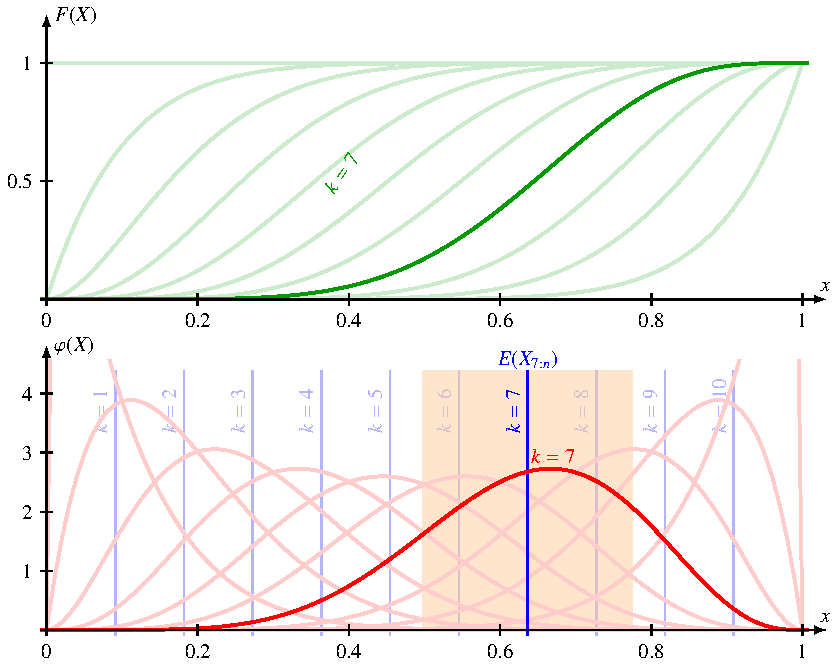
\includegraphics{chapters/040-rekursion/images/order.pdf}
\caption{Verteilungsfunktion und Wahrscheinlichkeitsdichte der
Ordnungsstatistiken $X_{k:n}$ einer gleichverteilung Zuvallsvariable
mit $n=10$.
\label{buch:rekursion:ordnung:fig:order}}
\end{figure}

%
% Die Beta-Funktion
%
\subsection{Die Beta-Verteilung
\label{buch:rekursion:subsection:beta-verteilung}}
Die Wahrscheinlichkeitsdichte, die im
Abschnitt~\ref{buch:rekursion:ordnung:section:ordnungsstatistik}
gefunden worden ist, ist nicht nur für ganzzahlige Exponenten
definiert.

\begin{figure}
\centering
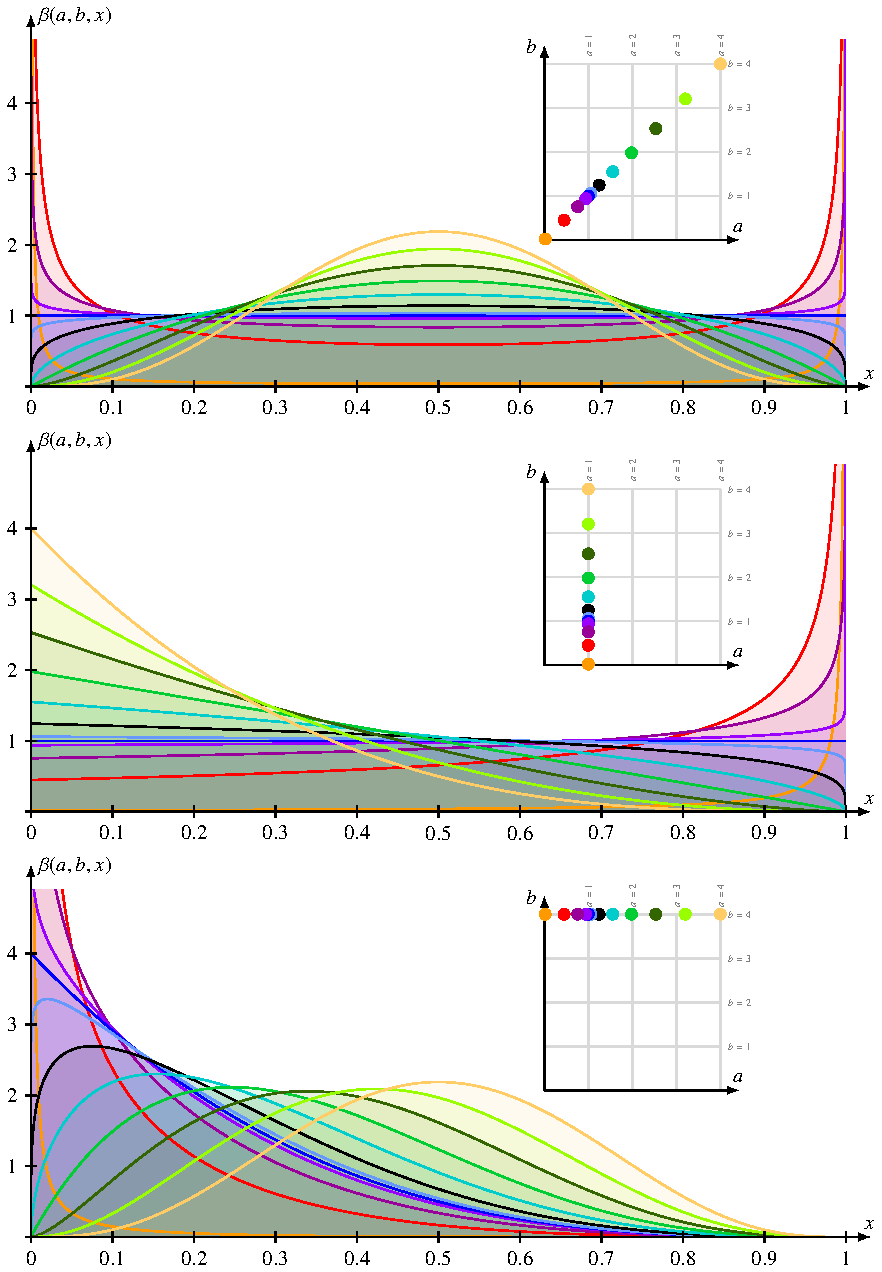
\includegraphics[width=0.92\textwidth]{chapters/040-rekursion/images/beta.pdf}
\caption{Wahrscheinlichkeitsdichte der Beta-Verteilung
$\beta(a,b,x)$
für verschiedene Werte der Parameter $a$ und $b$.
Die Werte des Parameters für einen Graphen einer Beta-Verteilung
sind im kleinen Quadrat rechts im Graphen
als Punkt mit der gleichen Farbe dargestellt.
\label{buch:rekursion:ordnung:fig:betaverteilungn}}
\end{figure}

\begin{definition}
\label{buch:rekursion:beta:def}
Die Beta-Verteilung ist die Verteilung mit der Wahrscheinlichkeitsdichte
\begin{equation}
\beta_{a,b}(x)
=
\begin{cases}
\displaystyle
\frac{1}{B(a,b)}
x^{a-1}(1-x)^{b-1}&\qquad 0\le x \le 1\\
0&\qquad\text{sonst.}
\end{cases}
\label{buch:rekursion:beta:eqn:def}
\end{equation}
\end{definition}

Die Beta-Funktion ist also die Normierungskonstante der Beta-Verteilung.
Die wichtigsten Kennzahlen der Beta-Verteilung wie Erwartungswert und
Varianz lassen sich alle ebenfalls als Werte der Beta-Funktion ausdrücken.

%
% Erwartungswert
%
\subsubsection{Erwartungswert}
Aus der Wahrscheinlichkeitsdichte \eqref{buch:rekursion:beta:eqn:def}
kann man jetzt auch den Erwartungswerte der $k$-ten Ordnungsstatistik
bestimmen.
Die Rechnung ergibt:
\begin{align*}
E(X_{k:n})
&=
\int_0^1 x\cdot k\binom{n}{k} x^{k-1}(1-x)^{n-k}\,dx
=
k
\binom{n}{k}
\int_0^1
x^{k}(1-x)^{n-k}\,dx.
\intertext{Dies ist das Beta-Integral}
&=
k\binom{n}{k}
B(k+1,n-k+1),
\intertext{welches man durch Gamma-Funktionen bzw.~durch Fakultäten wie in}
&=
k\frac{n!}{k!(n-k)!}
\frac{\Gamma(k+1)\Gamma(n-k+1)}{n+2}
=
k\frac{n!}{k!(n-k)!}
\frac{k!(n-k)!}{(n+1)!}
=
\frac{k}{n+1}
\end{align*}
ausdrücken kann.
Die Erwartungswerte haben also regelmässige Abstände, sie sind in
Abbildung~\ref{buch:rekursion:ordnung:fig:order} als blaue vertikale Linien eingezeichnet.

Für die Beta-Verteilung lässt sich die Rechnung noch allgemeiner 
durchführen.
Der Erwartungswert einer $\beta_{a,b}$-verteilten Zufallsvariablen $X$
ist
\begin{align*}
E(X)
&=
\int_0^1 x \beta_{a,b}(x)\,dx
=
\frac{1}{B(a,b)}
\int_0^1 x\cdot x^{a-1}(1-x)^{b-1}\,dx
=
\frac{B(a+1,b)}{B(a,b)}
=
\frac{a}{a+b}.
\end{align*}
Durch Einsetzen von $a=k+1$ und $b=n-k+1$ lassen sich die für die
Ordnungsstatistik berechneten Werte wiederfinden.

\subsubsection{Varianz}
Auch die Varianz einer Ordnungsstatistik lässt sich
einfach berechnen.
Dazu muss zunächst der Erwartungswert von $X_{k:n}^2$
bestimmt werden.
Er ist
\begin{align*}
E(X_{k:n}^2)
&=
\int_0^1 x^2\cdot k\binom{n}{k} x^{k-1}(1-x)^{n-k}\,dx
=
k
\binom{n}{k}
\int_0^1
x^{k+1}(1-x)^{n-k}\,dx.
\intertext{Auch dies ist ein Beta-Integral, nämlich}
&=
k\binom{n}{k}
B(k+2,n-k+1)
=
k\frac{n!}{k!(n-k)!}
\frac{(k+1)!(n-k)!}{(n+2)!}
=
\frac{k(k+1)}{(n+1)(n+2)}.
\end{align*}
Die Varianz wird damit
\begin{align}
\operatorname{var}(X_{k:n})
&=
E(X_{k:n}^2) - E(X_{k:n})^2
\notag
\\
&
=
\frac{k(k+1)}{(n+1)(n+2)}-\frac{k^2}{(n+1)^2}
=
\frac{k(k+1)(n+1)-k^2(n+2)}{(n+1)^2(n+2)}
=
\frac{k(n-k+1)}{(n+1)^2(n+2)}.
\label{buch:rekursion:ordnung:eqn:ordnungsstatistik:varianz}
\end{align}
In Abbildung~\ref{buch:rekursion:ordnung:fig:order} ist die Wurzel 
aus der Varianz der
Ordnungsstatistik $X_{k:n}$ für $k=7$ und $n=10$ als oranges
Rechteck dargestellt.

Die Varianz kann auch ganz allgemein für eine beliebige Beta-verteilte
Zufallsvariable bestimmt werden.
Dazu berechnen wir zunächst
\begin{align*}
E(X^2)
&=
\frac{1}{B(a,b)}
\int_0^1
x^2\cdot x^{a-1}(1-y)^{b-1}\,dx
=
\frac{B(a+2,b)}{B(a,b)}.
\end{align*}
Daraus folgt dann 
\[
\operatorname{var}(X)
=
E(X^2)-E(X)^2
=
\frac{B(a+2,b)B(a,b)-B(a+1,b)^2}{B(a,b)^2}.
\]

Die Formel~\eqref{buch:rekursion:ordnung:eqn:ordnungsstatistik:varianz}
besagt auch, dass die Varianz der $k$-ten Ordnungsstatistik proportional
ist zu $k((n+1)-k)$.
Dieser Ausdruck ist am grössten für $k=(n+1)/2$, die Varianz ist
also grösser für die ``mittleren'' Ordnungstatistiken als für die
extremen $X_{1:n}=\operatorname{min}(X_1,\dots,X_n)$ und
$X_{n:n}=\operatorname{max}(X_1,\dots,X_n)$.

